\section{Hip\'otesis de interacciones esenciales~\citep{he2006}}
Como hemos mostrado en la secci\'on \ref{sec:jeong} la correlaci\'on vista por Jeong es corroborada, sin embargo su hip\'otesis
de esencialidad debido centralidad por grado no responde al comportamiento real de las redes. He y sus colegas plantean una
hip\'otesis alternativa: La esencialidad se debe a la participaci\'on en interacciones esenciales y no esencialidad 
\textit{unitaria} como pensaba Jeong. Bajo esta hip\'otesis la regla de Centralidad-Letalidad se explica debido a que 
los hubs, al tener mayor cantidad de interacciones, tienen mayor probabilidad de pertenecer a una interacci\'on esencial.

El modelo de He considera dos condiciones de esencialidad: La prote\'ina participa en una interacci\'on esencial representada
en la red con una probabilidad $\alpha$ \'o la prote\'ina es esencial debido a alg\'un otro factor que la red no es capaz de
mostrar. As\'i la probabilidad de que un nodo de grado $k$ no participe en una interacc\'ion esencial es 
$(1-\alpha)(1-\alpha)\cdots(1-\alpha) = (1-\alpha)^k$ y la probabilidad de no ser esencial debido a otra raz\'on es $(1-\beta)$.
Luego, la probabilidad de no ser esencial es

\begin{align}
    \label{eq:ne}
    1-P_E(k) &= (1-\beta)(1-\alpha)^k\\
    \intertext{finalmente, la probabilidad de esencialidad es}
    P_E(k) &= 1 - (1-\beta)(1-\alpha)^k
\end{align}


A continuaci\'on evaluaremos la calidad de esta hip\'otesis a trav\'es de estimaciones de las probabilidades por dos m\'etodos 
descritos en el trabajo de He y colegas. Cabe se\~nalar que, para lo que resta del an\'alisis, la red AP-MS no ser\'a considerada,
debido a que \citet{he2006} hace referencia redes construidas a partir de asociaci\'on de complejos proteicos podr\'ian 
presentar comportamientos an\'omalos.

\subsection{M\'etodo de Ajuste}
Tomando el logaritmo a la ec. \ref{eq:ne} se tiene 
\begin{align}
    \ln(1-P_E(k)) &= k \ln(1-\alpha) + \ln(1-\beta)
\end{align}
es decir, una relaci\'on lineal entre el grado y la probabilidad de no-esencialidad. \citet{he2006} mensiona que, debido a que
a mayor grado $k$ es m\'as dificil encontrar nodos con grado $k$, por lo que para sus an\'alisis utiliza un umbral superior de
$k=10$. En este trabajo se ha considerado lo mismo. La figura \ref{fig:fit} muestra los resultados del ajuste lineal para 
nuestras redes. Debido al comportamineto irregular de la red Y2H (ver figura \ref{fig:y2h}) esta fue excluida del an\'alisis.

\begin{figure}[!ht]
    \centering
    \begin{subfigure}[b]{0.4\columnwidth}
        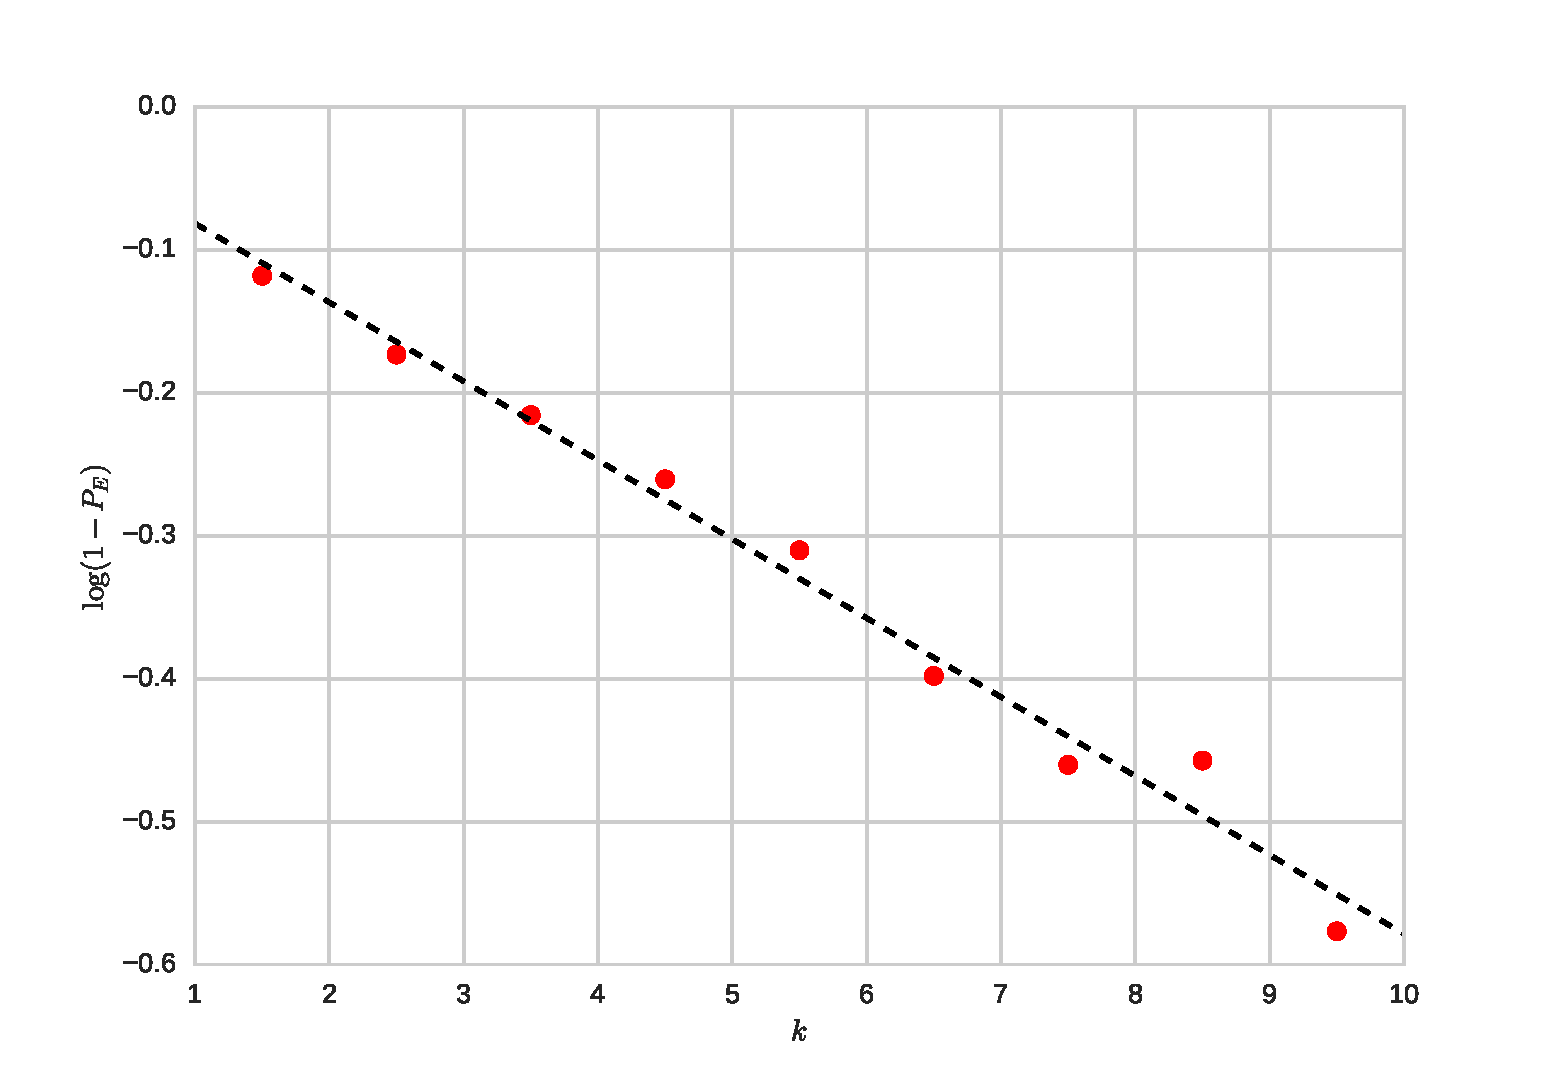
\includegraphics[width=\textwidth]{./schemes/yeast_LIT_Reguly.pdf}
        \caption{\label{fig:LITR}LIT\_Reguly}
    \end{subfigure}
    \begin{subfigure}[b]{0.4\columnwidth}
        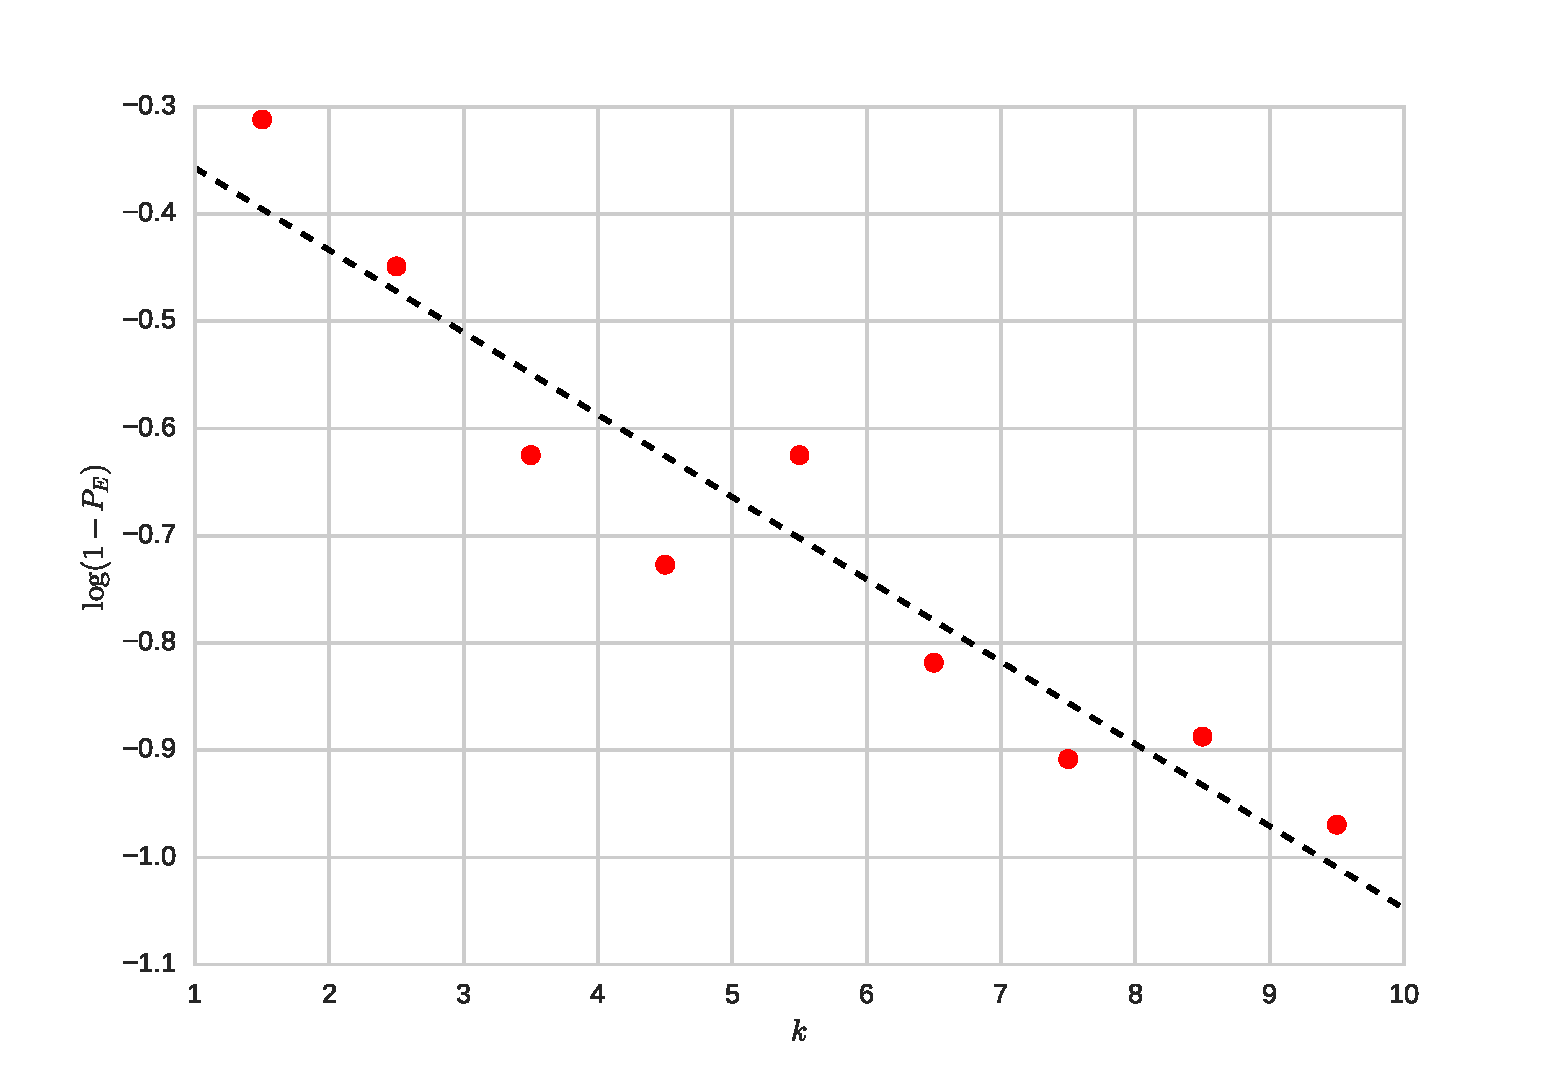
\includegraphics[width=\textwidth]{./schemes/yeast_LIT.pdf}
        \caption{\label{fig:LIT} LIT}
    \end{subfigure}
    \\
    \begin{subfigure}[b]{0.4\columnwidth}
        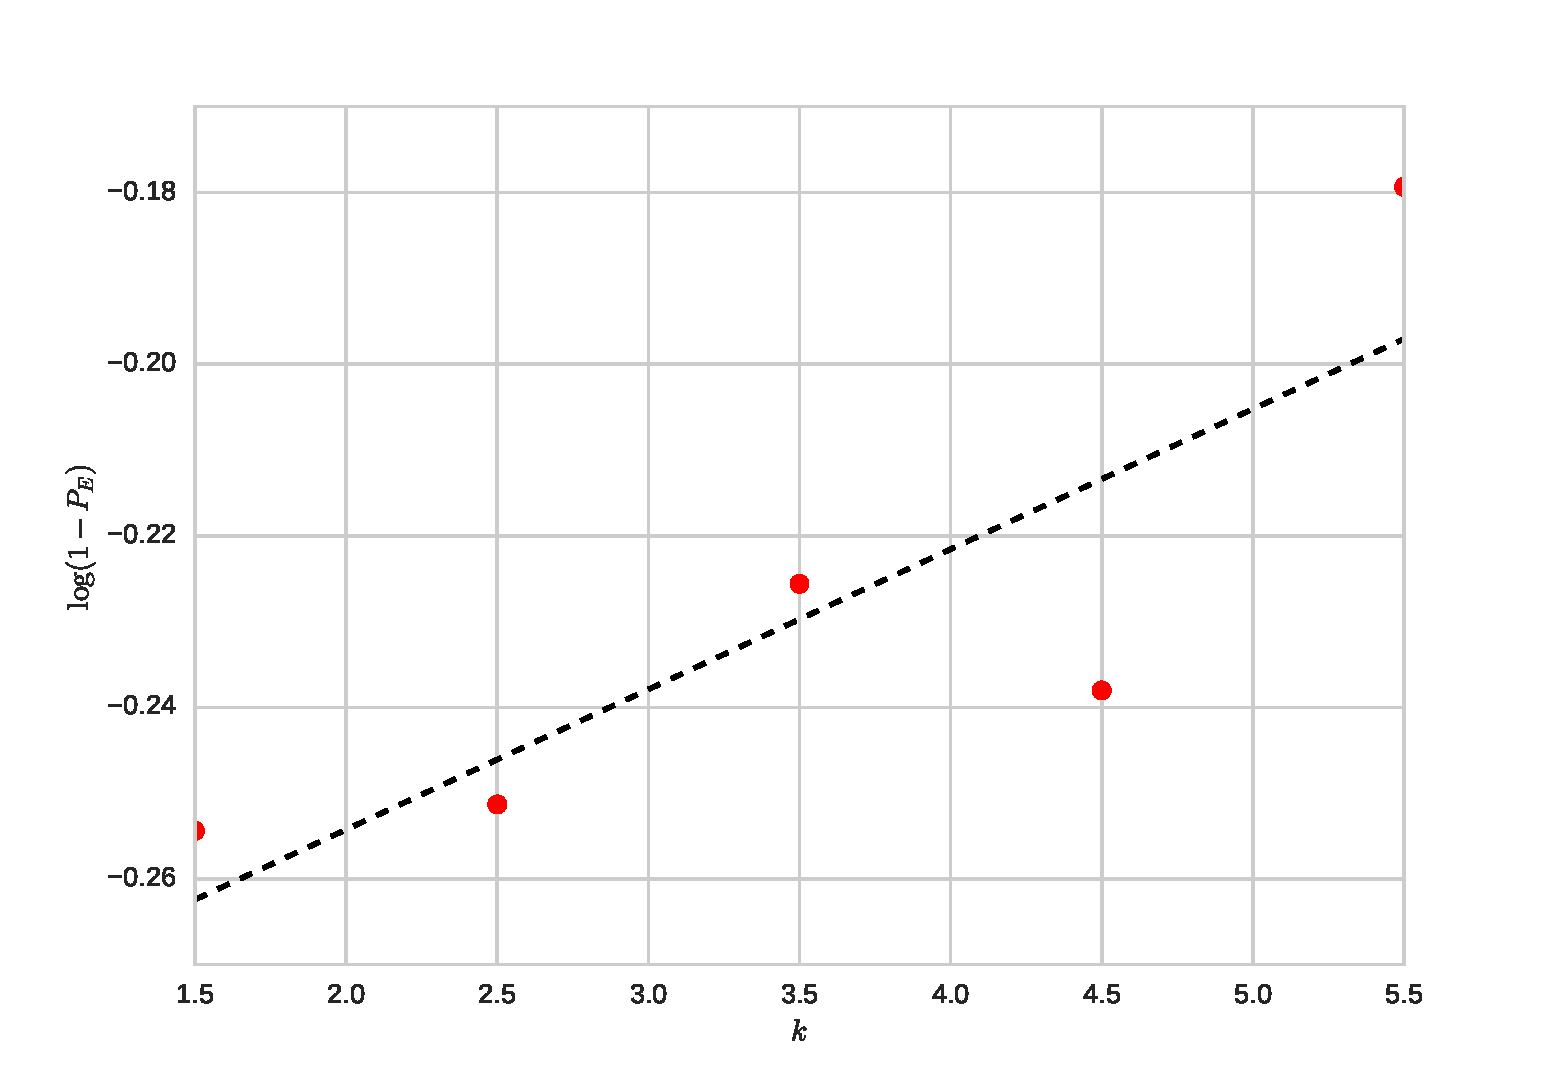
\includegraphics[width=\textwidth]{./schemes/yeast_Y2H.pdf}
        \caption{\label{fig:y2h} Y2H}
    \end{subfigure}
    \caption{\label{fig:fit} Ajustes lineales de las probabilidades de no-esencialidad y grado (ver ec. \ref{eq:ne}. 
    (a) $\alpha = 0.53 \pm 0.002 $ y $\beta = 0.26 \pm 0.017$; (b) $\alpha = 0.073 \pm 0.008$ y $\beta = 0.224 \pm 0.043$. 
    Debido al comportamiento irregular, Y2H ha sido excluida del an\'alisis.}
\end{figure}


\subsection{M\'etodo de simulaciones}

\subsection{Discuci\'on}
\begin{table}[!ht]
    \centering
    \caption{\label{tab:probas} Resumen de probabilidades estimadas para cada red a trav\'es de m\'etodo de ajuste
y simulaciones.}
    {\scriptsize
    \begin{tabularx}{.9\columnwidth}{XlccXccX}
        \hline\hline
        &               &  \multicolumn{2}{c}{Simulaci\'on}  &&  \multicolumn{2}{c}{Ajuste}          &      \\
        \cline{3-4} \cline{6-7}
        &               &   $\alpha$    & $\beta$            &&   $\alpha$       &       $\beta$     & \\
        \hline
        & LIT\_Reguly   &    &         && 0.053$ \pm$ 0.002  & 0.026 $\pm$ 0.017       &               \\
        & LIT           &    &         && 0.073 $\pm$ 0.008  & 0.244 $\pm$ 0.043       &               \\
        & Y2H           &    &         &&    ---             &   ---              &               \\
        \hline\hline
    \end{tabularx}
    }
\end{table}


\begin{table}[!ht]
    \centering
    \caption{\label{tab:pairs} Cantidad de pares totales o de igual caracteristica (ambos esenciales o ambos no esenciale)
    en comparaci\'on al valor estimado desprendido de la hipotesis de \citet{he2006}.}
    {\scriptsize
    \begin{tabularx}{.9\columnwidth}{XlccccX}
        \hline\hline
        &               & Pares   & Pares del   & \multicolumn{2}{c}{Pares esperados del mismo tipo }             \\ 
        \cline{5-6}
        &               & Totales & mismo tipo  & Simulaci\'on  &        Ajuste         &      \\
        \hline
 %       & AP-MS         & 11613 & 5924 & &  &            \\ 
        & LIT\_Reguly   & 10777   & 6187        &               &         5716          &               \\
        & LIT           & 1858    & 1059        &               &          963          &               \\
        & Y2H           & 2258    & 1493        &               &                       &               \\
        \hline\hline
    \end{tabularx}
    }
\end{table}
